%% LaTeX-Beamer template for KIT design
%% by Erik Burger, Christian Hammer
%% title picture by Klaus Krogmann
%%
%% version 2.1
%%
%% mostly compatible to KIT corporate design v2.0
%% http://intranet.kit.edu/gestaltungsrichtlinien.php
%%
%% Problems, bugs and comments to
%% burger@kit.edu

\documentclass[18pt]{beamer}

%% SLIDE FORMAT

% use 'beamerthemekit' for standard 4:3 ratio
% for widescreen slides (16:9), use 'beamerthemekitwide'

\usepackage{templates/beamerthemekit}
%\usepackage{templates/beamerthemekitwide}

\usepackage[utf8]{inputenc}

%% TITLE PICTURE

% if a custom picture is to be used on the title page, copy it into the 'logos'
% directory, in the line below, replace 'mypicture' with the 
% filename (without extension) and uncomment the following line
% (picture proportions: 63 : 20 for standard, 169 : 40 for wide
% *.eps format if you use latex+dvips+ps2pdf, 
% *.jpg/*.png/*.pdf if you use pdflatex)

\titleimage{btw_titel}

%% TITLE LOGO

% for a custom logo on the front page, copy your file into the 'logos'
% directory, insert the filename in the line below and uncomment it

%\titlelogo{mylogo}

% (*.eps format if you use latex+dvips+ps2pdf,
% *.jpg/*.png/*.pdf if you use pdflatex)

%% TikZ INTEGRATION

% use these packages for PCM symbols and UML classes
% \usepackage{templates/tikzkit}
% \usepackage{templates/tikzuml}

% the presentation starts here

\title[Interne Abnahme]{Mandatsverteilung für den Deutschen Bundestag}
\subtitle{Interne Abnahme}
\author{Manuel Olk}

\institute{Praxis der Softwareentwicklung, WS 2013/14}

% Bibliography

\usepackage[citestyle=authoryear,bibstyle=numeric,hyperref,backend=biber]{biblatex}
%\addbibresource{templates/example.bib}
\bibhang1em

\begin{document}

% change the following line to "ngerman" for German style date and logos
%\selectlanguage{english}
\selectlanguage{ngerman}

%title page
\begin{frame}
\titlepage
\end{frame}

%table of contents
\begin{frame}{Gliederung}
\tableofcontents
\end{frame}


\section{Zielsetzung}
\begin{frame}{Zielsetzung}
\begin{itemize}
	\item Wahlsystem komplex
	\item Programm dient dem Nachvollziehen der Wahlausgänge
	\item richtet sich an politisch Interessierte
\end{itemize}
\end{frame}

\section{Allgemeines zur Anwendung}
\subsection{Name}
\begin{frame}{Name}
\begin{itemize}
	\item Name dieser Anwendung ist OpenBundestagswahl
	\item Bild
\end{itemize}
\end{frame}


\subsection{Lizenz}
\begin{frame}{Lizenz}
\begin{itemize}
	\item GNU General Public License Version 3 (GPL V3)
	\begin{center}
		
\includegraphics[scale=0.5]{img/License-GPL3.png}
	\end{center}
	\item Garantierte Freiheit:
	\begin{itemize}
		\item Kostenlos für alle
		\item Jeder darf das Programm ändern
		\item Das Programm bleibt frei für alle
	\end{itemize}

	\item verwendete Bibliotheken:
	\begin{itemize}
		\item JFreeChart
		\item ICU
	\end{itemize}
\end{itemize}
\end{frame}

\subsection{Kenndaten und Leistungsmerkmale}
\begin{frame}{Plattformunabhängigkeit}
\begin{center}
	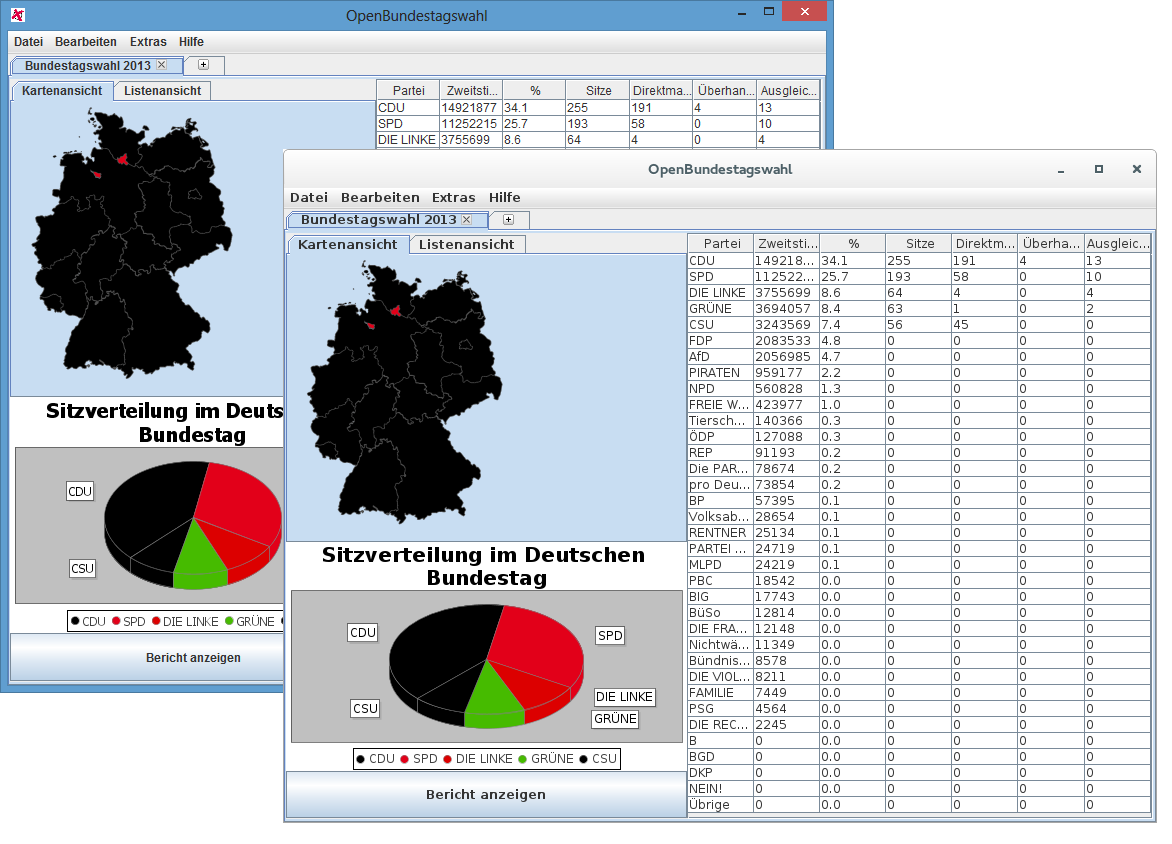
\includegraphics[scale=0.25]{img/app.png}
\end{center}
\begin{itemize}
	\item Windows
	\item GNU Linux
\end{itemize}
\end{frame}

\begin{frame}{Kenndaten und Leistungsmerkmale}
\begin{itemize}
	\item keine Internetverbindung notwendig
	\item Berechnung nach Wahlgesetz 2013
	\item unkomplizierte Bedienbarkeit
\end{itemize}
\end{frame}


\section{Funktionen}
\begin{frame}{Funktionen}
\begin{itemize}
	\item Auswertung der Sitzverteilung nach gesetzlicher Bestimmung
	\item Veranschaulichung der Ergebnisse durch eine anschauliche Oberfläche
	\item Generierung von Bundestagswahlen
	\item Gegenüberstellung von Wahlausgängen
	\item Import-/Exportmöglichkeit von Wahlen
	\item Stimmanzahländerungen
\end{itemize}
\end{frame}

\section{Live Demonstration}
\begin{frame}{Live Demonstration}
\begin{LARGE}
\begin{center}
	Nun folgt eine Live Demonstration
\end{center}
\end{LARGE}
\end{frame}


\section{Details zu Modulen}
\begin{frame}{Import/Export}
\begin{itemize}
	\item Wahlergebnisse von bundeswahlleiter.de
	\item Unterstützung von verschiedenen Zeichensätzen
	\item Verwendet Config für Informationen
\end{itemize}
\end{frame}


\begin{frame}{Mandatsrechner}
\begin{itemize}
	\item Berechnung nach Sainte-Lague/Schepers
	\item D'Hondt-Implementierung vorhanden
\end{itemize}
\end{frame}

\section{Rückblick und Erfahrungen}
\begin{frame}{Fachliche Erfahrungen}
\begin{itemize}
	\item Wasserfallmodell praktisch eingesetzt
	\item Neue Werkzeuge kennengelernt
	\item Relevanz von Testen erkannt
\end{itemize}
\end{frame}

\begin{frame}{Persönliche Erfahrung}
\begin{itemize}
	\item Gute Teamarbeit
	\item Gegenseitige Unterstützung und Motivation
\end{itemize}
\end{frame}

\section{Ausblick}
\begin{frame}{Ausblick}
\begin{itemize}
	\item Veröffentlichung auf GitHub
\end{itemize}
\begin{center}
	
\includegraphics[scale=0.3]{img/github-logo.png}
\end{center}

\end{frame}

\appendix

\begin{frame}{}

\begin{LARGE}
\begin{center}
	Vielen Dank für Ihre Aufmerksamkeit!
\end{center}
\end{LARGE}
\end{frame}

\end{document}
